\documentclass[11pt]{beamer}

\usetheme{metropolis}

\usepackage{graphicx}
\usepackage{physics}
\usepackage{adjustbox}
\usepackage{caption}
\usepackage{chemformula}
\usepackage{quoting}
\usepackage[style=chem-angew,backend=bibtex]{biblatex}
\bibliography{references}
%
% Choose how your presentation looks.
%
% For more themes, color themes and font themes, see:
% http://deic.uab.es/~iblanes/beamer_gallery/index_by_theme.html
%
\mode<presentation>
{
  \usetheme{default}      % or try Darmstadt, Madrid, Warsaw, ...
  \usecolortheme{default} % or try albatross, beaver, crane, ...
  \usefonttheme{default}  % or try serif, structurebold, ...
  \setbeamertemplate{navigation symbols}{}
  \setbeamertemplate{caption}[numbered]
  \setbeamerfont{footnote}{size=\tiny}
} 

\usepackage[english]{babel}
\usepackage[utf8]{inputenc}
\graphicspath{{image/}}

\AtBeginSection[]{
\begin{frame}{Outline}
  \tableofcontents[currentsection]
\end{frame}
}

\title{Chapter 9: Gaseous State}
\institute{Chemistry Department, Cypress College}
\date{Nov 16, 2022}

\begin{document}

\begin{frame}
  \titlepage
\end{frame}

\begin{frame}{Class Announcements}
  \textbf{Lab}
  \begin{itemize}
  \item Experiment 18 Boyle's Law
  \item Submit the lab reports and homework assignments
  \item Reminder - Need $70\%$ of laborator points to pass
    the course
  \end{itemize}

  \textbf{Lecture}
  \begin{itemize}
  \item Finish up Ch 8 and begin Ch 9
  \item Go over homework 11 (EC for students who present)
  \item Quiz and Homework assignment released Fri, Nov 18th at 3pm
  \end{itemize}
\end{frame}

\section{Defining Gas Pressure}

\begin{frame}{Smokey the Bear: Hot Air Balloon}
  \begin{center}
    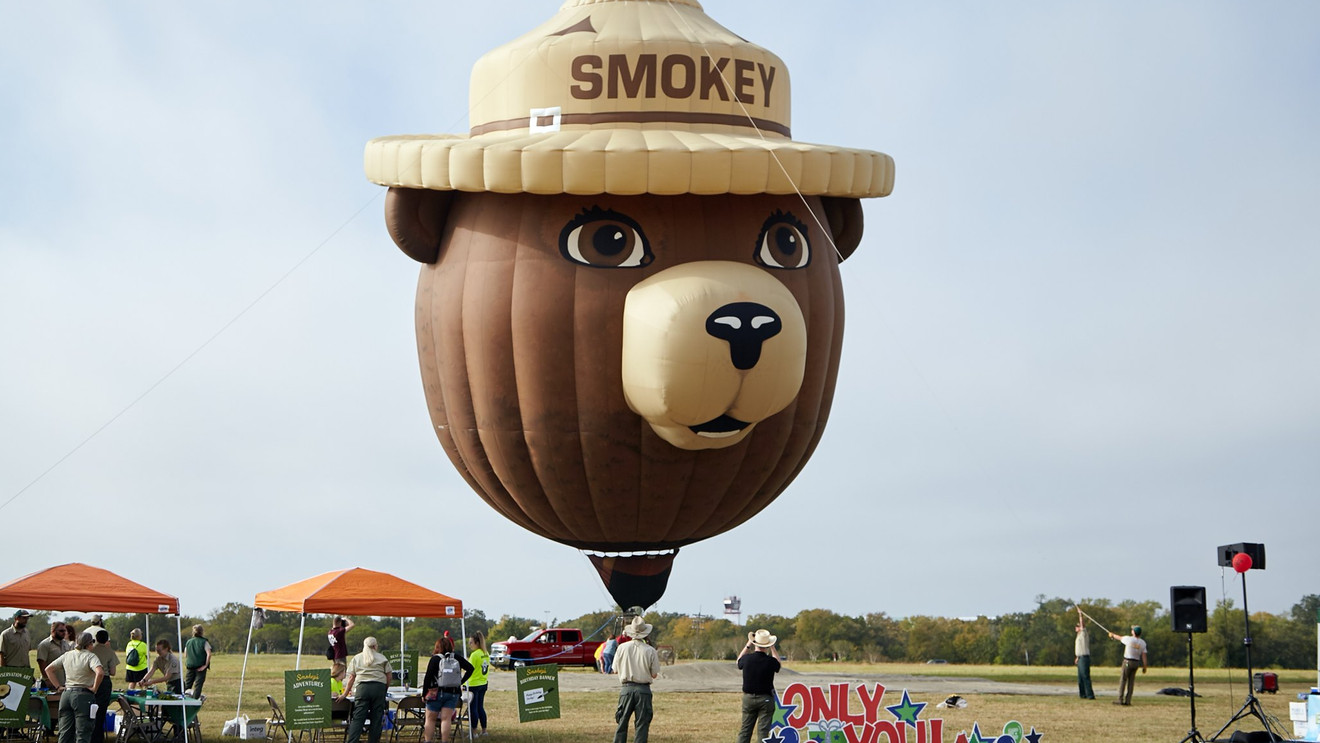
\includegraphics[scale=0.2]{smokey_air}
  \end{center}
  \textbf{Q:} How do air balloons float in the air?
\end{frame}

\begin{frame}{Defining Pressure}
  \begin{equation}
    P = \frac{F}{A}
  \end{equation}
  where $P$ is the pressure (N/m$^2$), $F$ is the force (Newton or N) acting on the area,
  and $A$ is the surface area (m$^2$)

  \textit{Common Units:} Psi, Torr, Pa, atm, mm Hg, and lb/in$^2$
\end{frame}

\begin{frame}{Measuring Pressure}
  \begin{center}
    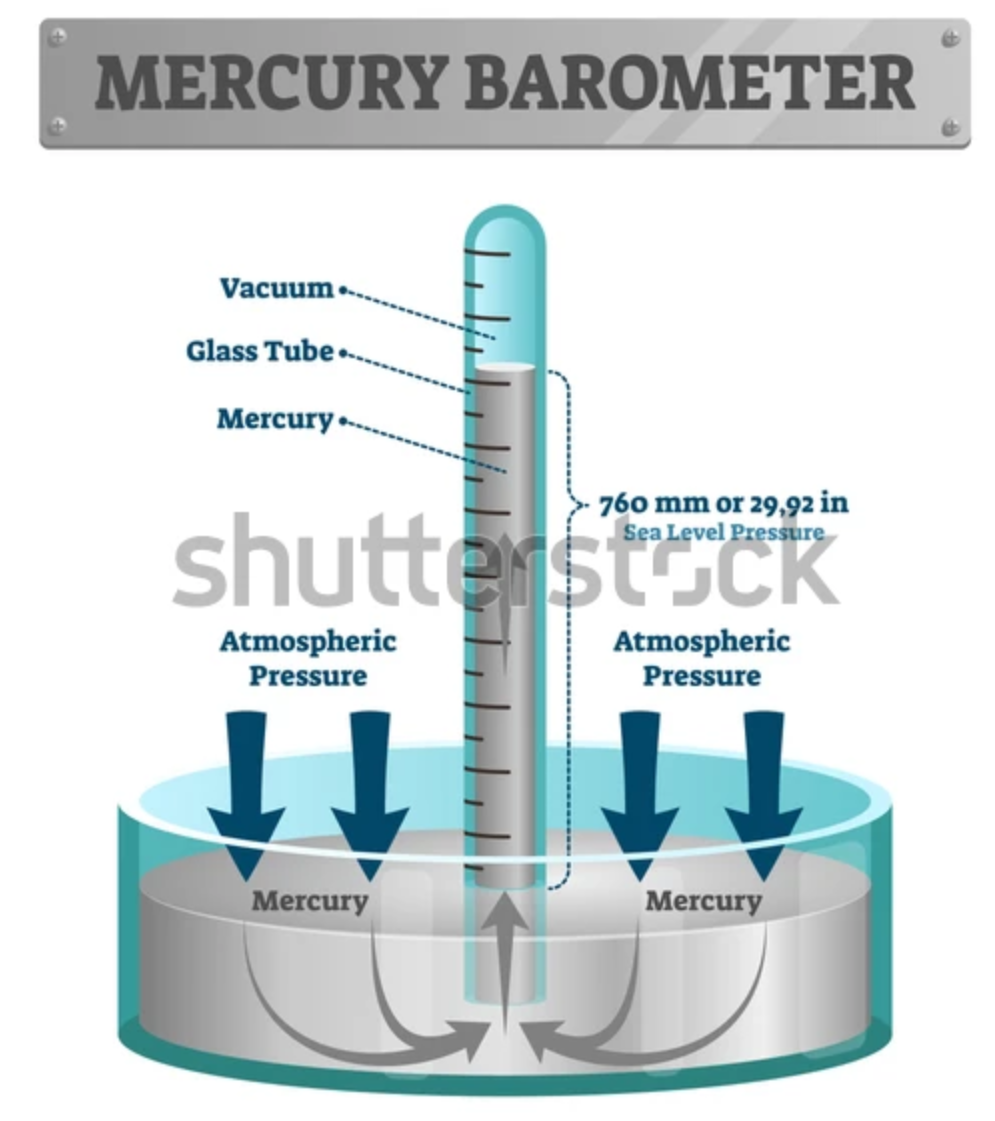
\includegraphics[width=0.6\linewidth]{merc_baro}
  \end{center}
\end{frame}

\begin{frame}{Common Pressure Units Conversion}
  \textit{Common Units:} Psi, Torr, atm, mm Hg, and lb/in$^2$
  \begin{align*}
    1 \text{atm} = & 760 \text{mm Hg} \\
    1 \text{atm} = & 101,325 \text{Pa} \\
    1 \text{atm} = & 14.7 \text{lb/in}^2
  \end{align*}
\end{frame}

\begin{frame}{Practice: Unit Conversion}
  Convert the following units:

  a) 845 Torr to atm

  b) 1.73 atm to Pa

  c) 32.1 lb/in$^2$ to atm

  \vspace{1in}
\end{frame}

\section{Gas Laws: Relationship P, V, and T}

\begin{frame}{Defn: Standard Temperature and Pressure}
  \textbf{Standard Temperature and Pressure (STP)}: the gas is at
  a given $0^\circ$C, 1 atm, and 22.414 L/mol
\end{frame}

\begin{frame}{Boyle's Law}
  For a given mole of gas, the pressure and volume are inversely
  proportional.
  \begin{align}
    PV = & \text{ constant} \\
    P_1V_1 = & P_2V_2
  \end{align}    
\end{frame}

\begin{frame}{Boyle's Law}
  \centering
  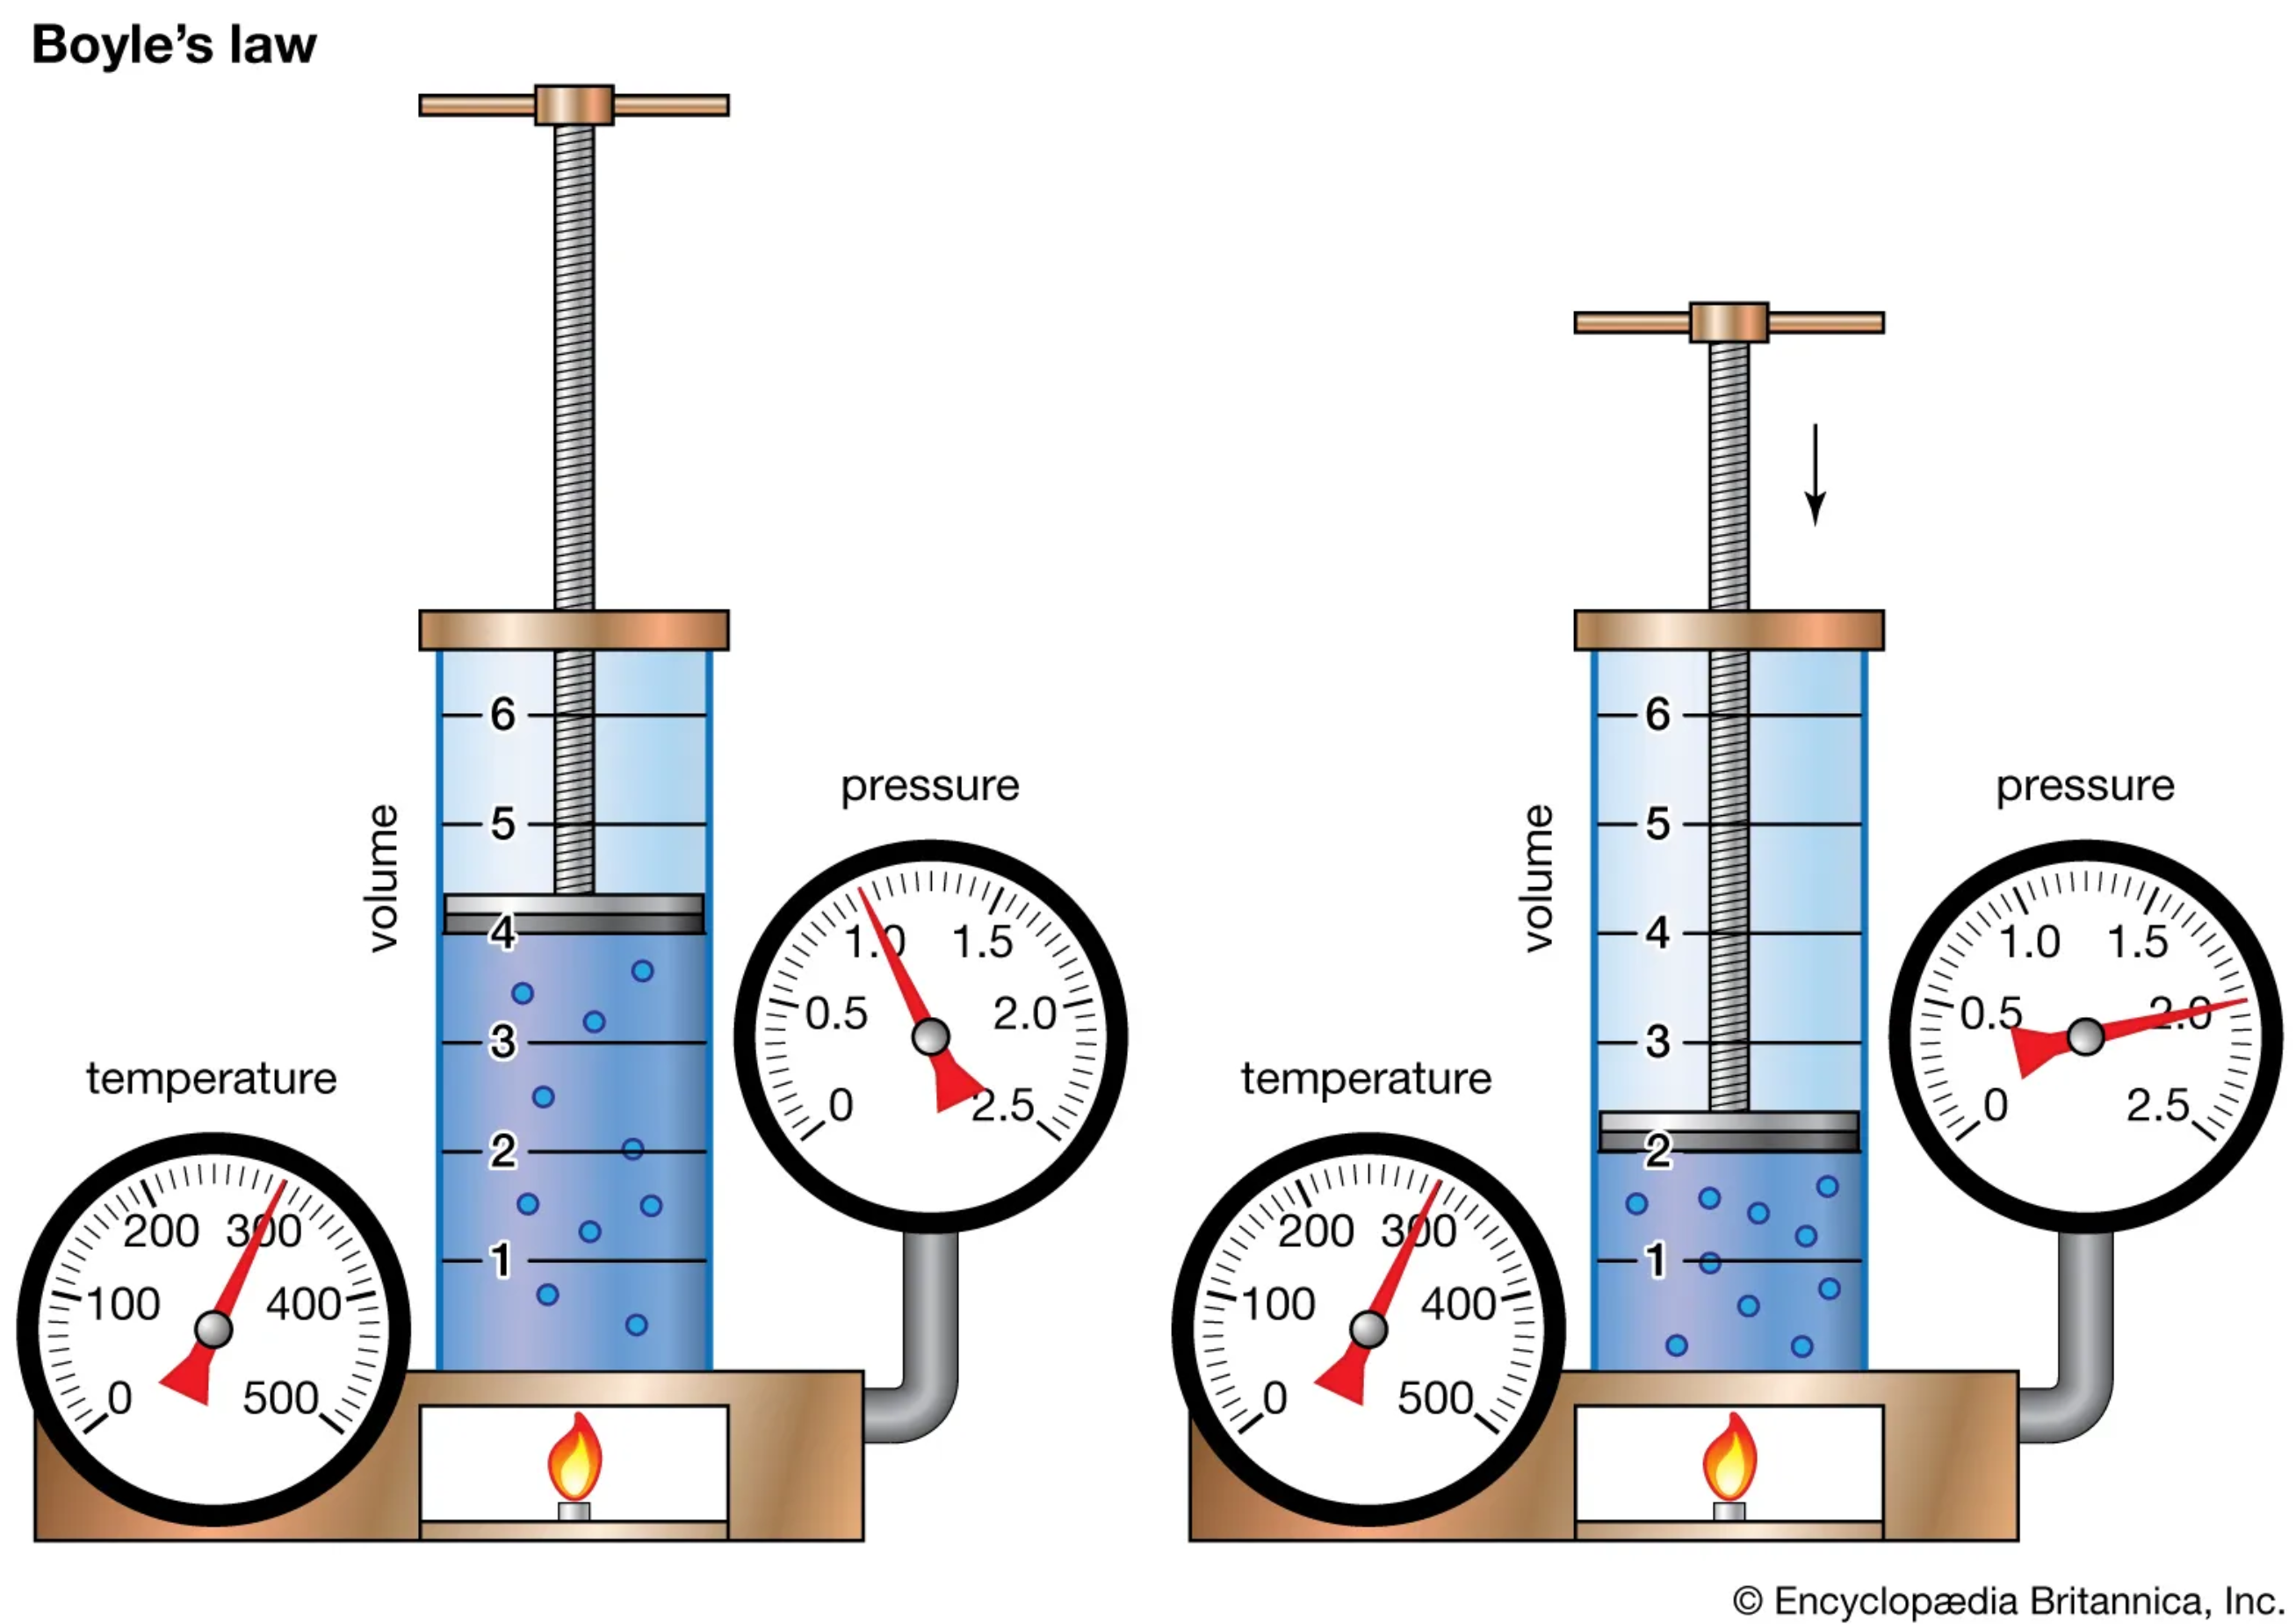
\includegraphics[width=\linewidth]{boyle_law}
\end{frame}

\begin{frame}{Graphing Boyle's Law}
  \centering
  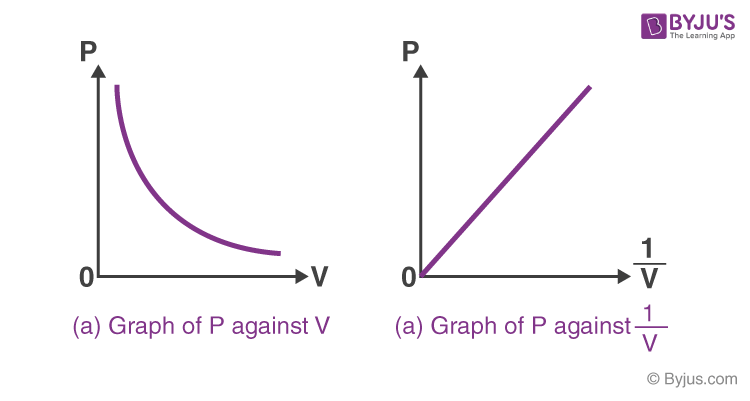
\includegraphics[width=0.9\linewidth]{boyle_graph}
\end{frame}

\begin{frame}{Practice: Boyle's Law}
  A balloon contains 510mL of helium when filled at 1.00atm. What would be
  the volume of the balloon if it were subjected to 2.50 atm of pressure?

  \vspace{1.5in}
\end{frame}

\begin{frame}{Charles' Law}
  For a given mole of gas, the volume and temperature are directly
  proportional
  \begin{align}
    \frac{V}{T} = & \text{ constant} \\
    \frac{V_1}{T_1} = & \frac{V_2}{T_2}
  \end{align}
\end{frame}

\begin{frame}{Charles' Law}
  \centering
  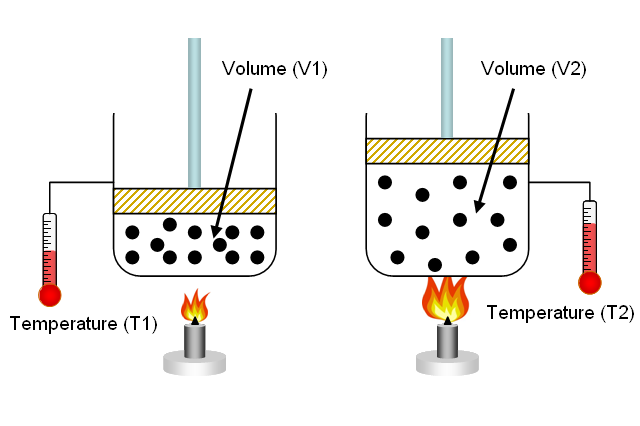
\includegraphics[width=0.9\linewidth]{charles_law}
\end{frame}

\begin{frame}{Graphing Charles' Law}
  \centering
  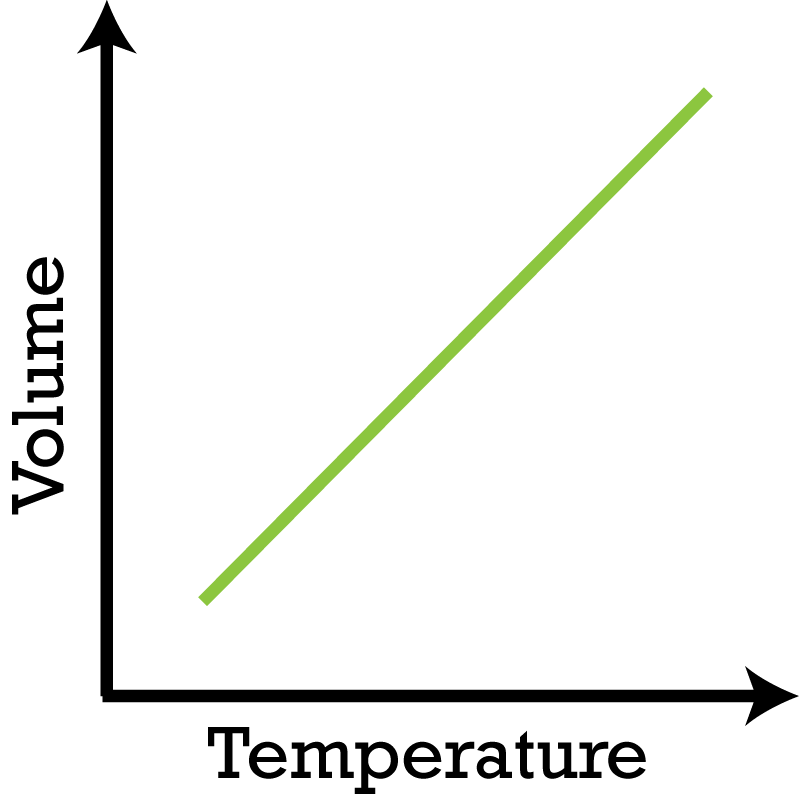
\includegraphics[width=0.6\linewidth]{charles_graph}
\end{frame}

\begin{frame}{Practice: Charles' Law}
  If a sample of chlorine gas occupies 50.0mL at 100.0$^\circ$C,
  what is its volume at 25.0$^\circ$C at constant pressure?
  
  \vspace{1.5in}
\end{frame}

\begin{frame}{Gay-Lussac's Law of Combining Volumes}
  In a reaction, the volume ratio of gas matches the mole ratio of
  the chemical equation

  2 H$_2$(g) + O$_2$(g) $\rightarrow$ 2 H$_2$O(g)
\end{frame}

\begin{frame}{Avogadro's Hypothesis}
  At constant temperature and pressure, the volume and moles of gas
  are directly proportional
  \begin{align}
    \frac{V}{n} = & \text{ constant} \\
    \frac{V_1}{n_1} = & \frac{V_2}{n_2}
  \end{align}
\end{frame}

\begin{frame}{Practice: Volume and Moles of Gas}
  If a 10.0L balloon contains 0.80 mol of a gas, what wil be the volume
  of a balloon that contains 0.20 mol of the gas if temperature and
  pressure remain constant?

  \vspace{1.5in}
\end{frame}

\end{document}
